\documentclass[10pt,dvipdfmx]{standalone}
% \documentclass[10pt,dvipdfmx,b5paper,papersize]{jsarticle}
\usepackage{tikz}
\usetikzlibrary{intersections, calc}
\usetikzlibrary{arrows.meta}
\usepackage{physics}


\begin{document}

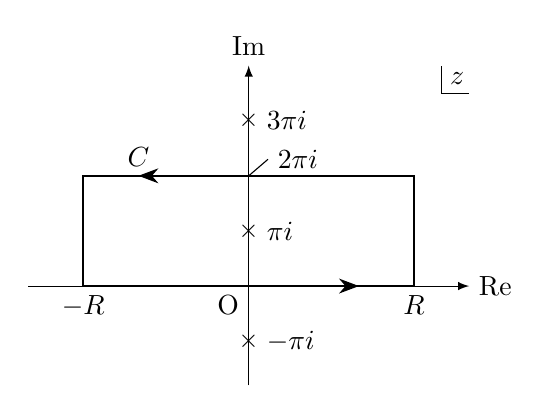
\begin{tikzpicture}[x=7mm,y=7mm,>=latex]
  % \small % 文字サイズ
  
  % 座標系
  \draw[->] (-4,0) -- (4, 0) node[right]{$\Re$}; % x軸
  \draw[->] (0,-1.8) -- (0, 4) node[above]{$\Im$}; % y軸
  \node(O) at (0,0) [below left]{O}; % 原点
  % 右上
  \def\ztx{3.5}
  \def\zty{3.5}
  \def\ztd{0.5}
  \draw (\ztx+\ztd,\zty) -- (\ztx,\zty) -- (\ztx,\zty+\ztd);
  \node at (\ztx,\zty) [above right=-0.5pt] {$z$};

  % 特異点
  \def\batsu{{\small $\times$}}
  % x軸上
  \foreach \y in {-1,...,1} {
    \node(O) at (0,2*\y+1) {\batsu};
  }
  % zeta = z
  % \path (1.5,3) coordinate (z) node{\batsu} node[right=2pt]{$\zeta=z$};

  % 四角
  \def\ax{3}
  \def\ay{2}
  \draw[thick] (-\ax,0) -- (-\ax,\ay) -- (\ax,\ay) -- (\ax,0) -- cycle;
  % 矢印
  \draw[arrows= {-Stealth[scale=1.5]}] (0,\ay) -- (-\ax+1,\ay);
  \draw[arrows= {-Stealth[scale=1.5]}] (0,0) -- (\ax-1,0);
  % C
  \node at (-\ax+1,\ay) [above]{$C$};

  % 座標
  \def\dx{0.8}
  \def\dy{0.5}
  \node at (\ax,0) [below] {$R$}; % 右
  \node at (-\ax,0) [below] {$-R$}; % 左
  \node at (0,3) [right=3pt] {$3\pi i$};
  \draw (0,2) -- (0.35,2.3) node[right] {$2\pi i$};
  \node at (0,1) [right=3pt] {$\pi i$};
  \node at (0,-1) [right=3pt] {$-\pi i$};
  
  % \draw (\ax,0) -- (\ax+\dx,\dy) node[above right=-3pt] {$\qty(N+\frac12)\pi $}; % 右
  % \draw (-\ax,0) -- (-\ax-\dx,\dy) node[above left=-3pt] {$-\qty(N+\frac12)\pi $}; % 左
  % \draw (0,\ay) -- (\dx,\ay+\dy) node[above right=-3pt] {$\qty(N+\frac12)\pi i$}; % 上
  % \draw (0,-\ay) --(\dx,-\ay-\dy) node[below right=-3pt] {$-\qty(N+\frac12)\pi i$}; % 下

  % テンプレ
  % \fill (2,1) coordinate (P) circle[radius=2pt] node[right=2pt] {P};

\end{tikzpicture}




\end{document}